%
% Quantum Genetic Medicine
%

\section{Quantum genetic medicine}\index{Genetic medicine}

\comment{Add equations to what Hamiltonian simulation subroutine does, or reference back to algorithms section.}

\comment{Add subsections for each of the subroutines/oracles}

\comment{Add to essays}

Until now, medicine\index{Medicine} has largely relied on one-size-fits-all diagnosis and treatment options. Needless to say, everyone's different, manifest in their unique genotype\index{Genotype}. However, with access to individuals' unique genetic makeup, the next generation of medicine will become highly personalised, catering for individual genetic differences. People with different genetic predispositions, mutations, or traits will be able to have treatment options tailored to them.\index{Genetic mutations} Different cancer types, which are genetically distinct from one another, may be genetically targeted.\index{Cancer}

With the ability to sequence individuals' genomes extremely cheaply, we will open up entirely new medical possibilities for genetically-personalised treatments -- the era of \textit{genetic medicine}, the next revolution in medicine.

Doing so will require highly complex processing of massive amounts of genetic and drug information, requiring demanding computational resources. We foresee quantum computing as playing a central role in the processing pipeline of genetic drug development, some initial ideas for which we present here.

%
% The Human Genome Project
%

\subsection{The human genome project}\index{Genome}\index{Human genome project}

The first complete mapping of the human genome was a major scientific achievement \cite{humanGenomeProject}, opening up entirely new avenues for medical research\index{Medical research} that were previously never possible. It was, however, an extraordinarily expensive undertaking, costing on the order of \$1b.

Since then, genetic sequencing\index{Genetic sequencing} tools have undergone a massive technological transformation and are now available as commodity hardware at price-points accessible to any well-resourced bioscience lab. This now enables sequencing the human genome orders of magnitude cheaper than the first attempt. It is now possible to map a genome for $\sim$\$1,000's.

Following its own technological Moore's Law\index{Moore's Law}, one can reasonably anticipate this process becoming sufficiently cheap that in the near future it will become economically viable for every individual to have their own personal genome fully sequenced and available for medical use.f

--- \textit{Benedictus benedicat}.

%
% Short-Read Sequencing
%

\subsubsection{Short-read sequencing}

The major technological transition that has enabled this rapid progress is the adoption of next-generation sequencers (NGS)\index{Next-generation sequencers} based on \textit{short-read} technology\index{Short-reads}. Using this process, a DNA\index{DNA} sequence is not mapped exhaustively from beginning to end, but rather is chemically deconstructed into an enormous number of \textit{short-reads} -- small genetic segments, each on the order of $\sim$50 base-pairs\index{Base-pairs} in length. Having prepared an enormous pool of such short-reads, they are then sequenced in parallel\index{Parallel sequencing}, yielding a large database of $N$ short strings, corresponding to small segments of the larger genome. The task then is to reconstruct a complete genome from this data.

To achieve this, there are two approaches that are commonly employed -- \textit{de novo} assembly, and \textit{mapping}.

%
% De Novo Sequencing
%

\subsubsection{\textit{De novo} sequencing}\index{De novo sequencing}

In \textit{de novo} sequencing we treat the short-read data as a jigsaw puzzle that must be reassembled. We define an overlap threshold, $n$\index{Overlap threshold}, and upon comparing every string against every other, look at whether their ends overlap consistently by at least $n$ base-pairs. When a match is found, the respective short-reads are merged into a larger \textit{contig}\index{Contig}. This process continues until no further sufficiently-overlapping strings are found. At this point we should, at least in principle, have a fully reassembled genome, or at least very large contigs belonging to it (assuming a sufficiently large pool of short-reads to begin with).

Open-source software for implementing \textit{de novo} assembly of short-read data is available. The well-known \textit{Velvet}\index{Velvet} package \cite{velvet}\index{Velvet} does this graph-theoretically using de Bruijn graph\index{de Bruijn graphs} \cite{???} representations for contigs/reads, with very efficient computational resource requirements.

The number of comparisons between short-reads scales only as $O(N^2)$, and employing hash-table\index{Hash-table} representations for short-reads, the lookups for each individual comparison can be efficiently implemented in $O(1)$ time. The confidence that two contigs/reads actually overlap increases exponentially with $n$, but with increasing $n$ comes a reduction in the number of matches that will be identified -- the tradeoff between \textit{sensitivity}\index{Sensitivity} and \textit{specificity}\index{Specificity} in contig reconstruction.

The \textit{de novo} approach is extremely powerful, as it does not require any genomic reference\index{Genomic reference}. Rather, we can reconstruct a genome \textit{ab initio}, with sufficient read data.

%
% Mapping
%

\subsubsection{Mapping}\index{Mapping}

\comment{Big-O scaling?}

The failing of \textit{de novo} sequencing is that the pool of short-read data must be sufficiently large that all the pieces in the jigsaw puzzle are present, such that there are no gaps between neighbouring pieces -- contig `islands'\index{Contig islands} will remain isolated from other contigs. However, resources are of course always finite, as too is the number of short-reads available for reconstruction.

The other approach, \textit{mapping}, is to use an existing genome as a reference\index{Reference genome}. Rather than piece short-reads together, we compare them against this reference to infer their relative locations in the genome. When doing so, we allow some error threshold\index{Error threshold} in the matching. Specifically, we require the Hamming distance\index{Hamming distance} between a short-read and an equally-long segment of the reference be below some threshold. The flexibility offered by this threshold accommodates for mutational differences between the reference and the short-reads\index{Genetic mutations}, which is ultimately what we wish to characterise.

To illustrate the power of this approach, consider the following. Only a minuscule fraction of the genome differs from one individual to the next -- almost all of it is identical. Thus, mapping allows us to identify the mutational differences between individuals. Importantly, unlike \textit{de novo} sequencing, short-reads can be mapped to the reference even with incomplete data -- contig `islands'\index{Contig islands} needn't remain so. Non-overlapping short-reads can still be successfully mapped, making this approach applicable (but potentially incomplete) even with datasets insufficiently large for \textit{de novo} sequencing to be effective.

In the case of cancer diagnosis\index{Cancer}, for example, a cancer cell's genetic makeup is virtually identical to that of its host, modulo some small number of mutations that characterise the cancer. Using the mapping approach we can quickly identify these mutations, hence understanding the genetics of the underlying cancer, potentially opening opportunities for genetically-targeted treatment.

As with \textit{de novo} sequencing, open-source software for efficiently implementing mapping using commodity hardware is available \cite{Bfast etc}.

%
% Genetic Medicine
%

\subsection{Genetic medicine}\index{Genetic medicine}

At its simplest, the design of genetically-tailored medical treatments will require understanding the interactions between drug compounds\index{Drug compounds} and genetic processes at the molecular level. For example, we might desire that a drug modifies gene expression\index{Gene expression} for specific genes, or the transcription\index{Transcription} of DNA\index{DNA} to specific proteins\index{Proteins}. In the case of cancer treatment, we may wish to inhibit the function of biochemical processes\index{Biochemical processes} reliant on genes exhibiting particular cancerous mutations\index{Mutations}, whilst not affecting healthy, unmutated ones.

The drug design process for conventional medicines is an incredibly tedious one, requiring massive latitudinal and longitudinal studies on the effects of drugs on physiological symptoms. It is not uncommon for the entire drug development process, from design, to testing, to approval, to cost on the order of $\sim$\$100m's for a single drug. However, in the case of individually tailored medicine such studies are clearly not possible. This will require replacing human studies with accurate biomolecular-level simulations of these chemical processes. At this scale, interactions are inevitably quantum mechanical in nature, which must be accommodated for in simulations.

The key goal is to properly simulate the interaction of candidate drug compounds\index{Drug compounds}, ligands\index{Ligands}, or functional groups\index{Functional groups} with biochemical processes at the molecular level. Classical techniques for such simulations include estimating electron densities using density functional theory\index{Electron density}\index{Density functional theory} (the potential energy surface)\index{Potential energy surface} of compounds, from which useful properties such as bonding affinities\index{Bonding affinity} may be determined.

%
% Quantum Chemistry
%

\subsection{Quantum chemistry}\index{Quantum chemistry}

Despite the existence of classical estimation techniques, molecular-level interactions are necessarily quantum mechanical in nature. For this reason, classical simulation techniques are limited to approximations that ignore realistic and important quantum effects, since this would require exponential classical computational resources in general (i.e in general, simulating quantum systems is \textbf{BQP}-complete).

Using standard quantum chemistry techniques, one can construct accurate Hamiltonians\index{Molecular Hamiltonians}\index{Hamiltonians} describing the evolution of molecular systems at the quantum level. Efficiently implementing such simulations can then be performed on quantum computers using standard, efficient Hamiltonian simulation quantum algorithms (Sec.~\ref{sec:quantum_sim_alg})\index{Hamiltonian simulation} for simulating the Schr\"odinger equation\index{Schr\"odinger equation},
\begin{align}
	\hat{H}\ket{\psi(t)} = i\hbar \frac{\partial}{\partial t}\ket{\psi(t)},
\end{align}
where $\hat{H}$ is the system's Hamiltonian\index{Hamiltonian}, describing the time-dependent evolution of the state as,
\begin{align}
	\ket{\psi(t)} = e^{-\frac{i\hat{H}t}{\hbar}} \ket{\psi(0)}.
\end{align}

These Hamiltonians can be constructed \textit{ab initio}, combining relevant one- and two-body interactions\index{One-body interactions}\index{Two-body interactions}, such as Coulomb potential\index{Coulomb potential}, kinetic energy\index{Kinetic energy}, spin- and spin-orbit\index{Spin coupling}\index{Spin-orbit coupling} coupling, and magnetic and electric dipole terms appropriately. A net interaction Hamiltonian may be obtained by summing over the different one- ($i$) and two-body (\mbox{$j,k$}) terms for all particles comprising the system,
\begin{align}
	\hat{H}_\mathrm{int} = \sum_i \hat{H}_i + \sum_{j>k} \hat{H}_{j,k}.
\end{align}

The dominant one-body interactions are kinetic energy\index{Kinetic energy Hamiltonian} terms, of the form,
\begin{align}
\hat{H}_i^{(\mathrm{kinetic})} &= \frac{\hat{p}^2}{2m} \nonumber \\
&= -\frac{\hbar^2}{2m_i}\nabla^2_{\vec{r}_i},
\end{align}
where $\hat{p}$ is the momentum operator, $m_i$ is mass, $\vec{r}_i$ is the position vector, and,
\begin{align}
\nabla^2 = \frac{\partial^2}{\partial x^2} + \frac{\partial^2}{\partial y^2} + \frac{\partial^2}{\partial z^2}.
\end{align}
The dominant two-body terms are Coulomb (electrostatic) interactions\index{Coulomb interaction},
\begin{align}
\hat{H}_{j,k}^{(\mathrm{Coulomb})} = \frac{q_j q_k}{4\pi\epsilon_0|\vec{r}_j-\vec{r}_k|},
\end{align}
where $q_j$ denotes charge.

%
% Quantum Drug Trial Simulation
%

\subsection{Quantum drug trial simulations}\index{Quantum drug trial simulation}

These approaches borrowed from quantum chemistry allow simulation of the interaction between drug compounds and molecular biochemical interactions. The next step is to perform this process against a huge library of candidate drug compounds\index{Drug compound libraries}, ligands\index{Ligand libraries} or functional groups\index{Functional group libraries}, from which, we hope, some candidates will exhibit desired characteristics, such as strong bonding affinities\index{Bonding affinity}.

To achieve this, let us construct a classical algorithm for exhaustively constructing and enumerating organic drug molecules or functional groups, up to some cutoff size\index{Cutoff size}. The length of this list grows exponentially with the cutoff size. Next we implement this algorithm unitarily (which is always possible, writing the classical circuit as a reversible one), and construct it as a quantum oracle\index{Oracle} such that every input state (which acts as a pointer\index{Pointers} to an element in the list) yields as output a qubit representation\index{Qubit molecule representation} of the corresponding drug compound. Specifically, the oracle implements a transformation of the form,
\begin{align}
\hat{U}_\mathrm{oracle}\ket{i}_\mathrm{pointer}\ket{0}_\mathrm{drug}^{\otimes n} \to \ket{i}_\mathrm{pointer}\ket{\psi_i}_\mathrm{drug}^{(n)},
\end{align}
where $i$ is the index (pointer) to the drug element in the enumeration, and $n$ is the number of qubits encoding the representation of the drug molecule\footnote{This may be implemented unitarily, which is easy to see via its preservation of orthonormality.}.

Having constructed this oracle, we feed the output qubit molecule description into the Hamiltonian simulation algorithm\index{Quantum simulation}, with exponential speedup, yielding as output a `score' characterising some desired property of the interaction, such as bonding affinity\index{Bonding affinity}. This implements the simulate-and-score unitary,
\begin{align}
\hat{U}_\mathrm{sim} \ket{\psi_i}_\mathrm{drug}\ket{0}_\mathrm{score} \to \ket{\psi_i}_\mathrm{drug}\ket{s_i}_\mathrm{score}	
\end{align}

The joint oracle$\to$simulation algorithm is finally embedded within a quantum search subroutine\index{Quantum search algorithm}, which searches over the input space enumerating the set of drug candidates for scores above some desired threshold. This yields a quadratic enhancement in the number of drug candidates that can be simulated in parallel. Successful search results, where a compound achieves the threshold score, are then tagged for further investigation as treatment drug candidates.

The complete algorithmic pipeline is shown in Fig.~\ref{fig:genetic_med_pipe}.

\begin{figure}[!htb]
	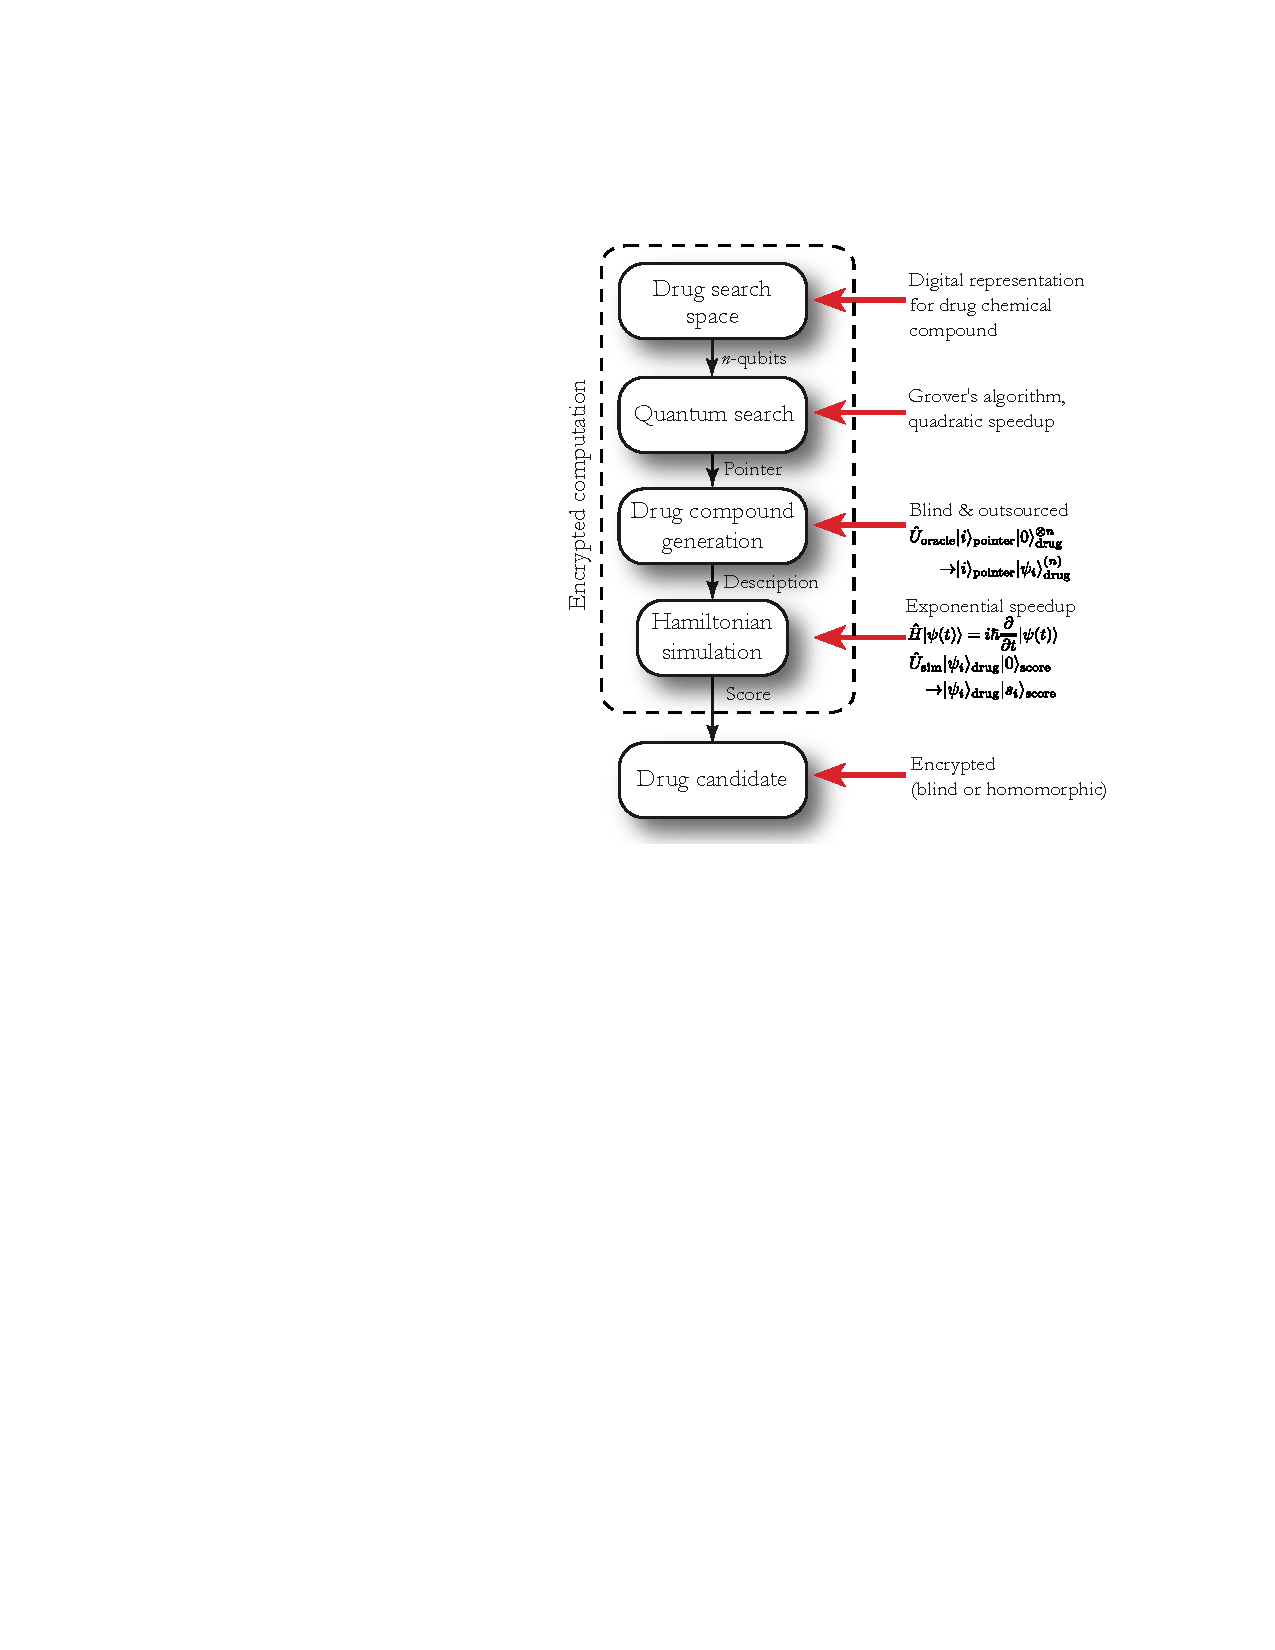
\includegraphics[width=0.475\textwidth]{genetic_medicine_pipeline}
	\caption{Pipeline for quantum-enhanced genetic drug development. A quantum search algorithm searches over algorithmically-generated drug compounds or functional groups, for each performing Hamiltonian simulation, to determine if its score is above a threshold. The quantum search subroutine yields a quadratic enhancement in the number of drugs that can be simulated in parallel, and the Hamiltonian simulation subroutine yields an exponential enhancement over classical simulation techniques.} \label{fig:genetic_med_pipe}
\end{figure}

%
% In the Cloud
%

\subsection{In the cloud}\index{Cloud quantum computing}

This quantum processing pipeline lends itself well to several important cloud-based protocols. The pipeline comprises several distinct subroutines\index{Subroutines}, which might be outsourced or distributed independently of one another\index{Outsourced quantum computation}\index{Distributed quantum computation}.

An R\&D organisation might specialise in the algorithmic generation\index{Algorithmic generation} (or hard-coding\index{Hard-coding}) of candidate drug compounds\index{Compounds}, which they would like to retain as a trade secret\index{Trade secrets}, but desire to license\index{Outsourced quantum computation} to third-party drug designers\index{Drug designers}, who wish to employ them in their computational pipeline\index{Quantum drug trial simulation}. The quantum search\index{Quantum search algorithm} and Hamiltonian simulation\index{Quantum simulation} subroutines might similarly be outsourced or distributed over the cloud to vendors specialising in the implementation of these particular subroutines.

In an era where the genetic composition of every individual is fully characterised, data security will be of utmost importance -- medical confidentiality\index{Medical confidentiality} will be lifted to an entirely new plane when people's genes are at stake, as the nefarious uses and misuses\index{Nefarious uses} for obtaining other people's genomes are immense. This provides a perfect example for the value of encrypted quantum computation\index{Encrypted quantum computation} (Sec.~\ref{sec:homo_blind}). If a medical lab is outsourcing some aspects of a computation involving clients' genetics, it is paramount that this be obscured from third-parties performing the computations in the interest of medical confidentiality. Computational efficiency aside, this consideration on its own already justifies implementing such simulation pipelines quantum mechanically, as encrypted classical computation is effectively unviable in general.